\documentclass[10pt]{beamer}
\setbeamertemplate{note page}[plain]
\usepackage[utf8]{inputenc}
\usepackage[T1]{fontenc}
\usepackage[utopia]{mathdesign}
\usetheme[progressbar=frametitle]{metropolis}


\usepackage{amsmath,amssymb}
\usepackage[spanish, mexico]{babel}
\usepackage{graphicx}
\usepackage{xcolor,xparse}
\usefonttheme[onlymath]{serif}
\makeatother
\renewcommand{\thefootnote}{\ifcase\value{footnote}\or$\dagger$\or
$\ast$\or\$\or\#\or\ddagger\or$\therefore$\fi}
\makeatletter

\title{Calefacción de una placa con sistema de control}
\subtitle{Final transferencia de calor }
\date{\today}

\author{Patricio Whittingslow -- 55423 \\ Luís Cretton}

\begin{document}
{
\begin{frame}[plain]
  \vspace{-4.3cm}
               
  {\Large \scshape{\textrm{Gimballed EDF propelled VTVL vehicle \\
  design and control}} \par}
  \vspace{0cm}
  { \textrm{Patricio Whittingslow --- 55423 \\ Luis Cretton --- 55555 }}
  
\end{frame}
}

\begin{frame}{Objetivo}
    \begin{itemize}
        \item Tecnología central para el desarrollo aeroespacial futuro
        \item Desarrollo de vehículo plataforma para ensayos a pequeña escala
    \end{itemize}

    \hspace{0.7cm}
    \begin{figure}[htb]
        \centering
        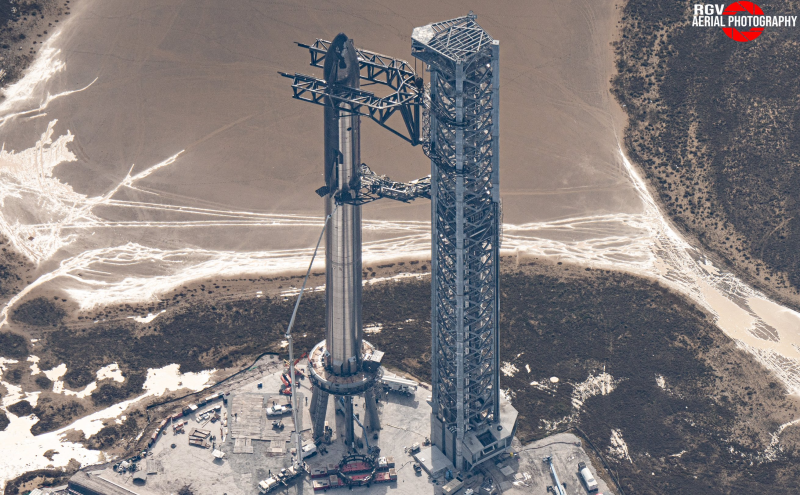
\includegraphics[width=0.8\linewidth]{fig/starship.png}
        \caption{Starship: referente en tecnología de vehículos orbitales reutilizables.}
        \label{fig:starship}
    \end{figure}
\end{frame}

\begin{frame}{Estado del arte}
    \begin{itemize}
        \item Tecnología monorrotor fijo tiene uso amplio
    \end{itemize}

    \begin{figure}[htb]
        \centering
        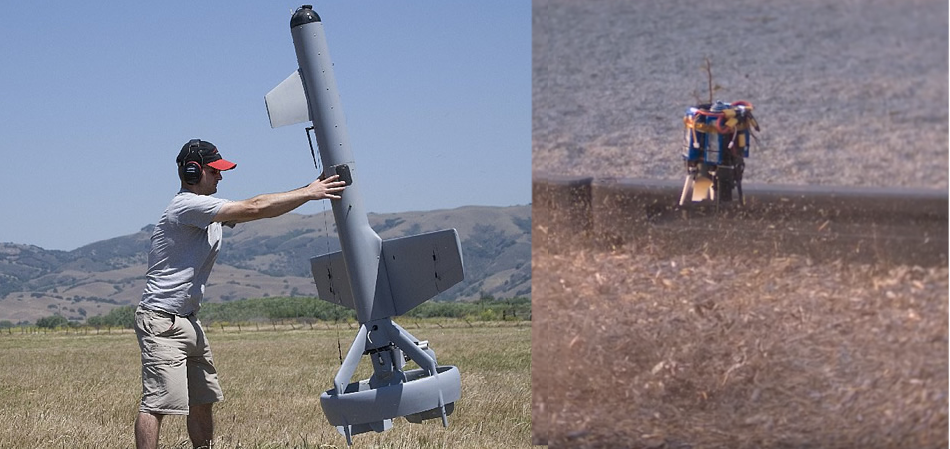
\includegraphics[width=0.8\linewidth]{fig/vbat_icarus.png}
        \caption{Dos vehículos VTVL eléctricos modernos. ``VBat'' (Izq.) y ``\href{https://hackaday.com/2018/08/31/single-rotor-drone-a-thrust-vectoring-monocopter/}{Ikarus}''.}
        \label{fig:vbat_icarus}
    \end{figure}
\end{frame}

\begin{frame}{Estado del arte}
    \begin{itemize}
        \item Tecnología monorrotor para empuje vectorial siendo usado por la ESA para ensayar algoritmos de control.
    \end{itemize}

    \begin{figure}[htb]
        \centering
        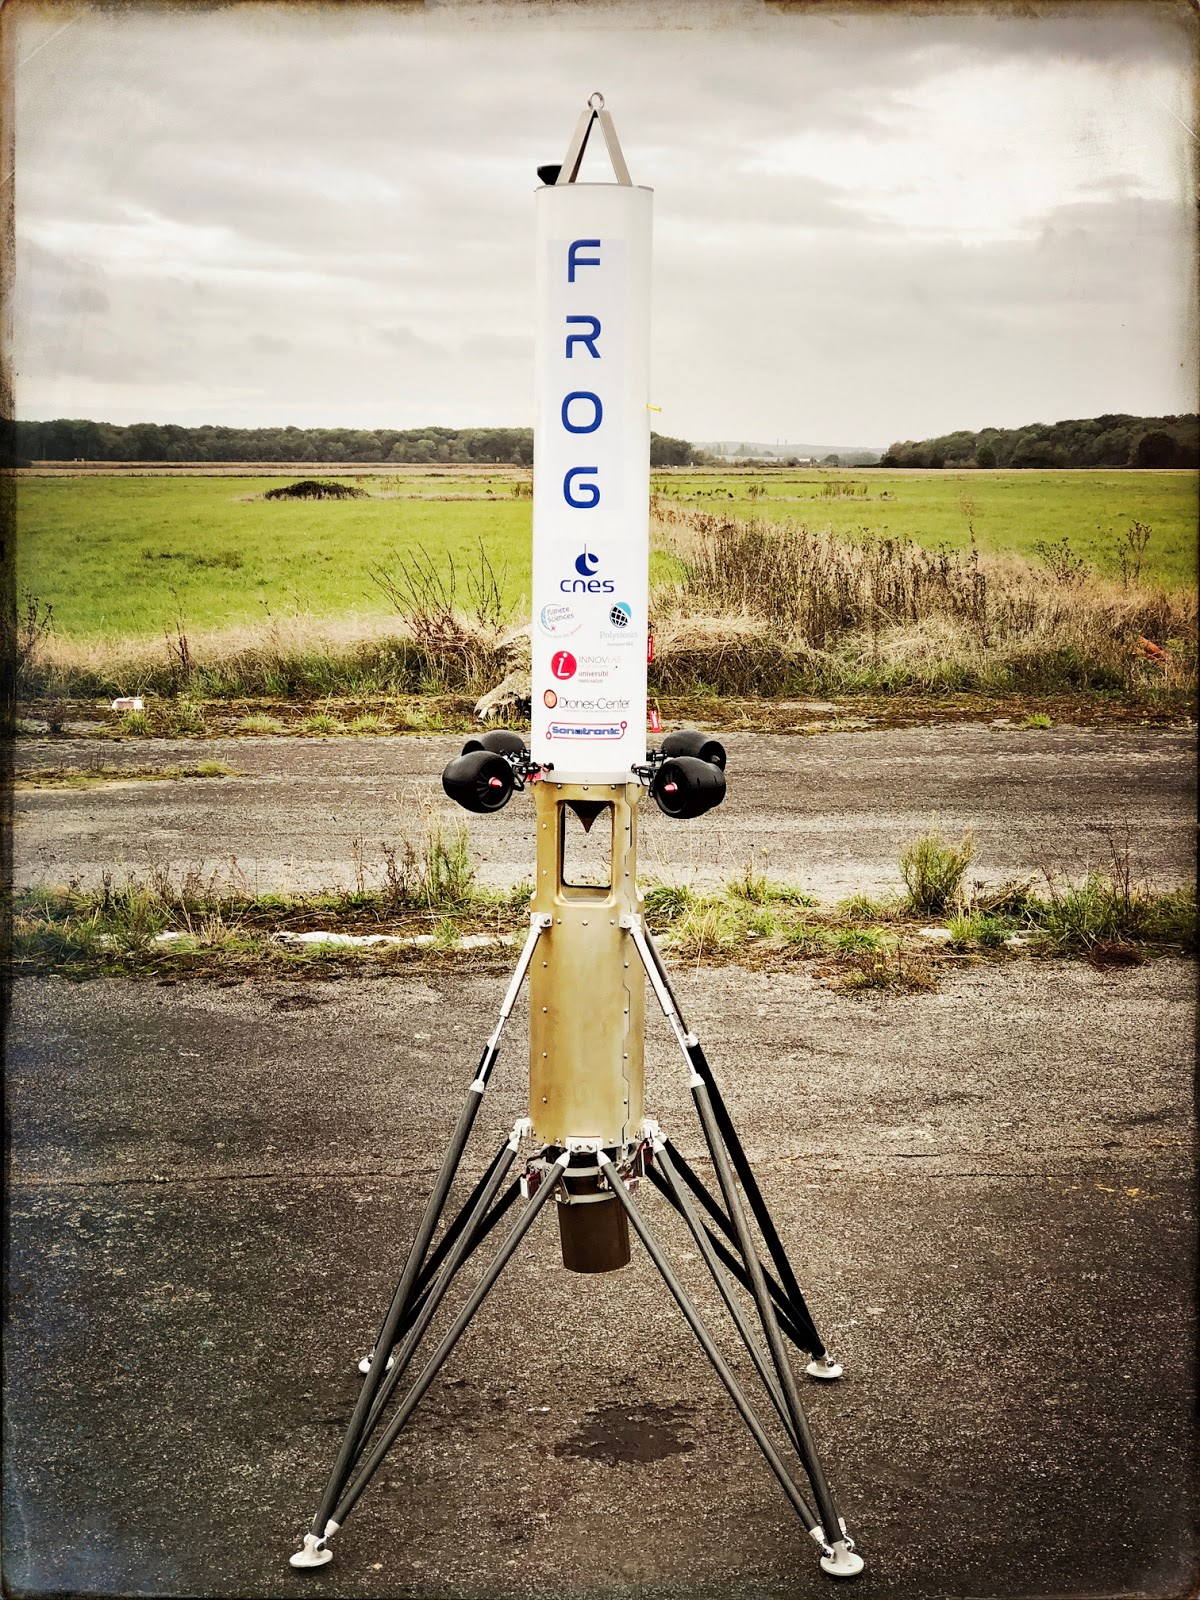
\includegraphics[height=6cm]{fig/frog_esa.jpg}
        \caption{FROG de la ESA. Plataforma de ensayo de sistemas.}
        \label{fig:frog_esa}
    \end{figure}
\end{frame}

\end{document}